\section{Muestreo natural, Instantáneo y S\&H}

En esta sección se desea analizar el comportamiento de diferentes técnicas de muestro:

\begin{itemize}
    \item Muestreo natural.
    \item Muestreo instantáneo.
\end{itemize}

\noindent bajo diferentes condiciones.

\subsection{Introducción teórica}
Previo a analizar lo solicitado en la consigna de este informe, se hará un breve desarrollo matemático con tal de justificar la subsecuente línea argumentativa. En la consigna de este informe se nos plantea el siguiente esquema:


\begin{figure}[H]
  \centering
  
\includegraphics[width = \textwidth]{Imagenes/5_Muestreo/esquema_inicial.pdf}
  \caption{Esquema planteado.}
  \label{fig: esquema simplificado del muestreo}
\end{figure}

\noindent donde potencialmente una etapa o varias etapas han de ser \emph{bypassed}. Sin embargo, en este análisis inicial, se analizará al sistema:

\begin{figure}[H]
  \centering
  \includegraphics[width = \textwidth]{Imagenes/5_Muestreo/Esquema_general.pdf}
  \caption{Esquema simplificado del muestreo.}
  \label{fig: esquema simplificado del muestreo}
\end{figure}

\noindent es decir, no se tendrán en cuenta al filtro anti-alias (FAA) y del filtro de recuperación (FR).

\subsubsection{Muestreo instantáneo}

Con tal de analizar el fenómeno en cuestión debemos de analizar la operatoria que realiza el sistema sobre la señal de entrada al realizar un muestreo instantáneo.

\begin{figure}[H]
  \centering
  \includegraphics[width = \textwidth]{Imagenes/5_Muestreo/Muestreo_inst.pdf}
  \caption{Modelado del muestreo instantáneo.}
  \label{fig: modelado del muestreo instantaneo}
\end{figure}

\noindent Donde es posible modelar al mismo en dos etapas. En primer lugar se multiplica la señal de entrada por un tren de deltas, obteniendo:

\begin{equation}
x^{*}(t) = x(t) \cdot \sum_{n \in \mathbb{Z}} \delta(t-n/f_s)
\end{equation}

\noindent Transformando ambos miembros:

\begin{equation}
X^{*}(f) = X(f) * \sum_{n \in \mathbb{Z}} f_s \delta(f-nf_s)
\end{equation}

Luego, se introduce ese tren de deltas a un sistema que toma una delta y devuelve un pulso de igual altura; es decir, un sistema que dispone de la siguiente respuesta impulsiva:

\begin{equation}
h(t) = \Pi \left(\frac{t-\tau/2}{\tau}\right)
\end{equation}

\noindent Por lo que su respuesta en frecuencia corresponde con:

\begin{equation}
H(f) = \tau \cdot sinc(\tau f) \cdot e^{-j2\pi f \tau/2}
\end{equation}

\noindent De este modo, la relación entrada salida se condice con:

\begin{equation}
Y(f) = \left[X(f) * \sum_{n \in \mathbb{Z}} f_s \delta(f-nf_s)\right] 
\cdot \tau \cdot sinc(\tau f) \cdot e^{-j2\pi f \tau/2}
\end{equation}

\noindent En particular, siendo:

\begin{equation}
\tau = \frac{1}{2f_s}
\end{equation}

\begin{equation}\label{eq: muestreo inst}
Y(f) = \left[X(f) * \sum_{n \in \mathbb{Z}} \delta(f-nf_s)\right] 
\cdot \frac{1}{2} \cdot sinc\left(\frac{f}{2f_s}\right) 
\cdot e^{-j2\pi \frac{f}{4f_s}}
\end{equation}

\noindent De este modo vemos que se replica el espectro original en cada múltiplo de $f_s$, mientras que, al mismo tiempo, se encuentra modulado por una sinc (notar que la exponencial debido al desplazamiento temporal del pulso únicamente aporta un desfasaje, pero no modifica el módulo).

\subsubsection{Muestreo natural}
En segundo lugar se dispone del muestreo natural. Esta operatoria puede ser modelada bajo el siguiente esquema:

\begin{figure}[H]
  \centering
  \includegraphics[width = \textwidth]{Imagenes/5_Muestreo/Muestreo_nat.pdf}
  \caption{Modelado del muestreo natural.}
  \label{fig: modelado del muestreo natural}
\end{figure}

\noindent es decir, como el producto de la señal de entrada por una señal rectangular de frecuencia $f_s$, duty cycle $D$, que varía entre un nivel unitario y cero:

\begin{equation}
y(t) = x(t) \cdot m(t)
\end{equation}

\noindent Al mismo tiempo, esta señal de muestreo se puede escribir a partir de relaciones ya conocidas:

\begin{equation}
m(t) = \Pi \left(\frac{t-D(1/2f_s)}{D(1/f_s)}\right) 
* \sum_{n \in \mathbb{Z}} \delta(t-n/f_s)
\end{equation}

\noindent Transformando:

\begin{equation}
M(f) = D \cdot \frac{1}{f_s} \cdot sinc\left(\frac{D f}{f_s}\right) 
\cdot e^{-j2\pi (f/f_s) D/2}
\cdot \sum_{n \in \mathbb{Z}} f_s \delta(f-nf_s)
\end{equation}

\begin{equation}
= \sum_{n \in \mathbb{Z}} D \cdot sinc(nD) 
\cdot e^{-j2\pi nD/2} \cdot \delta(f-nf_s)
\end{equation}

\noindent Por lo que:

\begin{equation}\label{eq: muestreo natural}
Y(f) = X(f) * M(f) 
= X(f) * \sum_{n \in \mathbb{Z}} 
D \cdot sinc(nD) \cdot e^{-j2\pi nD/2} \cdot \delta(f-nf_s)
\end{equation}

Donde resulta interesante resaltar que nuevamente se obtiene una replicación del espectro original en cada múltiplo de $f_s$ junto con una modulación de una sinc; sin embargo, aquí la modulación del espectro depende de que réplica proviene la componente, no de la frecuencia resultante.

\subsubsection{Muestreo con S\&H}
En última instancia se tiene al muestreo con S\&H (i.e. sin re-muestrear con el AS). De este modo, a la salida se este subsistema se observa el seguimiento de la señal mientras se esta sampleando (idealmente), alternado con el periodo de hold. Este tipo de muestreo puede caracterizarse mediante:

\begin{figure}[H]
  \centering
  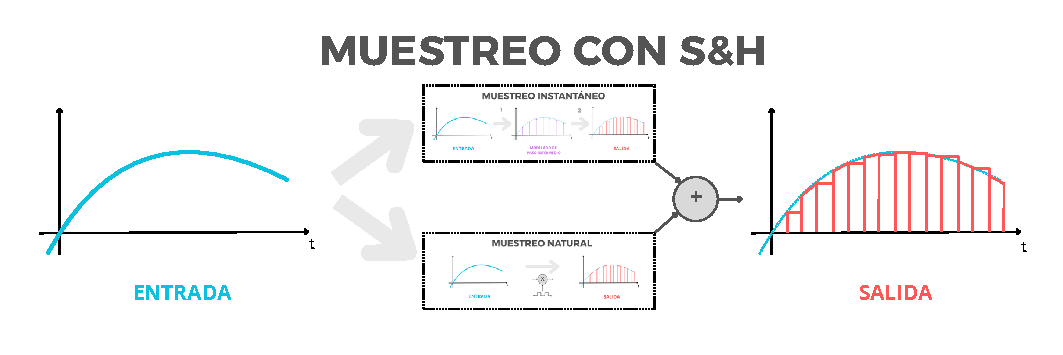
\includegraphics[width = \textwidth]{Imagenes/5_Muestreo/Muestreo SH.pdf}
  \caption{Modelado con S\&H.}
  \label{fig: muestreo con SH}
\end{figure}

\noindent donde se ha de realizar un defasaje temporal de 180° sobre la señal cuadrada empleada en la multiplicación del muestreo natural. De este modo, siendo que este defasaje se traduce en negar la transformada de Fourier, el espectro de este muestreo se caracteriza por:

\begin{align*}
    Y(f) &= Y_{inst} - Y_{nat} =  \left[X(f) * \sum_{n \in \mathbb{Z}} \delta(f-nf_s)\right] 
\cdot D_{hold} \cdot sinc(D_{hold} f/f_s) \cdot e^{-j2\pi D_{hold} f/2f_s} \\
&- X(f) * \sum_{n \in \mathbb{Z}} 
D_{sample} \cdot sinc(nD_{sample}) \cdot e^{-j2\pi nD_{sample}/2} \cdot \delta(f-nf_s)
\end{align*}

\noindent Donde se denota que se  dispone de la misma replicación que los casos anteriores, sin embargo la dependencia para con ambos muestreos evita un generalización mas precisa.


\subsubsection{Filtros}
En el análisis previo se omitieron los filtros con tal de simplificar el desarrollo. Sin embargo, para es relevante estudiar el efecto que tienen estos para con la relación entrada-salida.

En primera instancia se dispone del filtro anti-alias, este filtro tiene como finalidad, como su nombre lo indica, de acotar en frecuencia la señal de entrada tal que no se produzca aliasing. En otras palabras, su fin es restringir el espectro de la señal de entrada a un ancho $f_c$, tal que $fc < \frac{f_s}{2} = f_{nyquist}$.

Por otro lado se tiene al filtro recuperador. Este sistema esta orientado a eliminar las réplicas generadas por la discretización de la señal (ver ecuaciones (\ref{eq: muestreo inst}) y (\ref{eq: muestreo natural})) dejando únicamente la \emph{banda base}.

Este esquema es uno simplificado, orientado a la resolución del trabajo presentado, exciten variantes que no se abarcarán aquí (por ejemplo, los filtros en cuestión no necesariamente han de ser pasa-bajos).

En particular, la cátedra propuso un filtro que dispone de la siguiente respuesta en frecuencia:

\begin{figure}[H]
    \centering
    \begin{subfigure}{0.48\textwidth}
        \centering
        \includegraphics[width=\textwidth]{Imagenes/5_Muestreo/filtro_mag.png}
        \caption{Magnitud.}
        \label{fig: magnitud resp en frec filtro}
    \end{subfigure}
    \hfill
    \begin{subfigure}{0.48\textwidth}
        \centering
        \includegraphics[width=\textwidth]{Imagenes/5_Muestreo/filtro_pha.png}
        \caption{Fase}
        \label{fig: fase}
    \end{subfigure}
    \caption{Respuesta en frecuencia de FAA \& FR}
    \label{fig: respuesta en frec FAA y FR}
\end{figure}

\noindent Donde se observa una falencia patológica del análisis realizado: no existe un pasa-bajos ideal. En función de la finalidad de cada filtro surgen ciertos problemas. 

Por un lado, si el FAA no es ideal y se dispone de una señal cuyo ancho de banda excede la frecuencia de Nyquist, el aliasing es inevitable. Por fortuna, si se dispone de un filtro de alto orden es posible reducir los efectos de este fenómeno tal que no sean un problema (con ciertas consideraciones).

Por otro lado, la no-idealidad del FR conlleva que la señal de salida disponga de contenido espectral de otras bandas que no sean la base. Cuyo impacto puede ser nuevamente reducido bajo una selección acorde del filtro.

Finalmente, la figura \ref{fig: fase} da cuenta de otro hecho a tener en consideración: los filtros alteran la fase de la señal de un modo no lineal. De este modo, la integridad de la señal en cuestión se vera inherentemente afectada.

\subsection{Marco experimental}
Dadas las señales:

\begin{align*}
    {x_3}_{(t)} &= A \cdot \cos(2\pi \cdot f_{in}\cdot t) & \\
    {x_4}_{(t)} &= \text{onda cuadrada, con } T=2/f_{in} \ \& \ DC=75\% &
\end{align*}

\noindent con $f_{in} = 15kHz$. Se piden analizar diferentes configuraciones:

\subsubsection{Salida proporcional}
En primera instancia debemos analizar la frecuencia de muestreo ($f_s$), amplitud ($A$) y duty cycle ($D$) para muestrear ambas señales bajos esquemas y obtener una señal con mínima distorsión a la salida.


Comencemos con la señal $x_3$. Siendo esta una señal acotada en banda (dispone únicamente de 1 armónico en $f_{in}$) reconocemos que el filtro anti-alias únicamente modifica levemente la fase de la señal. Por otro lado, el filtro recuperador potencialmente puede alterar el comportamiento de la señal en función de la frecuencia de muestreo, pues $f_p = 22.05kHz$, siendo posible que alguna réplica caiga en la banda de paso; por lo que la elección de esta ha de ser con esta consideración. 

Independientemente del tipo de muestreo, la réplica de la bandas laterales se encuentran en $f_{rep} = f_{s} - f_{in}$ (en general analizamos lo que ocurre con las frecuencias positivas y como son señales reales sabemos que ocurrirá lo mismo en el semi-eje negativo), por lo que es posible que $f_{rep} < f_p$ y se disponga de este armónico a la salida. Sin embargo, es posible diferenciar aqui el comportamiento de ambos tipos de muestreo. 

Previo a entender las restricciones, veamos que ocurre si realizamos un muestreo de $f_s =32kHz$ y quitando el filtro de recuperación. El espectro de las señales de entrada y salida en el caso de muestreo instantáneo con duty del $50\%$ se condice con:



\begin{figure}[H]
  \centering
  \includegraphics[width = 0.7 \textwidth]{Imagenes/5_Muestreo/a_inst_fs_32k_fin_15k_D_50.pdf}
  \caption{Espectro de señales de entrada y salida | $f_s = 32kHz$ - $D=50\%$ | Muestreo instantáneo.}
  \label{fig: 5a_ins fs 32k D 50}
\end{figure}

\noindent Por otro lado en el caso del muestreo natural ocurre algo semejante:

\begin{figure}[H]
  \centering
  \includegraphics[width = 0.7 \textwidth]{Imagenes/5_Muestreo/a_nat_fs_32k_fin_15k_D_50.pdf}
  \caption{Espectro de señales de entrada y salida | $f_s = 32kHz$ - $D=50\%$ | Muestreo natural.}
  \label{fig: 5a_nat fs 32k D 50}
\end{figure}

\noindent EstOS espectroS claramente no son satisfactorios, dado que disponemos de armónicos en la banda de paso del filtro de recuperación. Sin embargo, nos permiten ver las carácterísticas explicadas en los distintos muestreos: por un lado la Figura \ref{fig: 5a_ins fs 32k D 50} exhibe la modulación del espectro por una sinc del muestreo instantáneo, mientras que la del muestreo natural, Figura \ref{fig: 5a_ins fs 32k D 50}, denota que esa modulación no es función de la frecuencia sino de la base de la que deriva la imagen. De este modo, el ejemplo mostrado denota el rol del duty cycle en esta cuestión.

La modulación por la sinc esta dada por las relaciones:

\begin{align*}
\text{Muestreo instantáneo:} \quad 
&D\cdot\text{sinc}\left(\frac{D \cdot f}{f_s}\right) \\[8pt]
\text{Muestreo natural:} \quad 
& D\cdot\text{sinc}(nD)
\end{align*}

 \noindent si se aumenta el duty cycle, se puede analizar que la modulación de la sinc se produce más rápidamente, por lo que se eliminarán las componentes de mayor frecuencia más rápidamente. En el caso de la muestreo instantáneo, esto también afecta a la componente en banda base; por ejemplo con $D=0.5$, en $f_{nyquist} =f_s/2$ hay una atenuación a $0.9$ de la componente original ($10\%$ de atenuación). De este modo, reducir el duty cycle restringe como se ve afectada la banda base. Por otro lado, en el muestreo natural, la banda base no depende del duty cycle, por lo que aumentar este restringe las componentes de más alta frecuencia sin afectar la amplitud en la banda de interes.  

 Siendo que se dispone de únicamente una línea espectral para la señal $x_3$, resulta conveniente un duty cycle del $50\%$. 

 Por otro lado, la elección de la frecuencia de muestreo se a de hacer de manera tal que la imagen de la banda lateral no caiga dentro de la banda de paso del filtro de recuperación. Sin embargo, el criterio de elección una vez dado esta selección aún no esta del todo definido. Dada la plantilla del filtro, sabemos que por encima de $f_a=44.1kHz$ la atenuación supera los $40dB$, si se considera que esta es la ganancia necesaria para que las componentes sean tomadas como nulas, la frecuencia debería de ser tal que $f_s - f_{in} < f_a=44.1kHz$, por lo que $f_s > 59kHz$. Otro criterio por ejemplo, que la atenuación sea mayor que 12dB (la ganancia a de caer por debajo de $1/4$), esto ocurre en $f = 28kHz$, por lo que se obtiene $f_s >43kHz$. Las señales temporales se corresponden con:
 
 \begin{figure}[H]
    \centering
    \begin{subfigure}{0.48\textwidth}
        \centering
        \includegraphics[width=\textwidth]{Imagenes/5_Muestreo/a_inst_fs_43_45_k_fin_15k_D_50.pdf}
        \caption{$f_s =43kHz$}
        \label{fig: 43kHz}
    \end{subfigure}
    \hfill
    \begin{subfigure}{0.48\textwidth}
        \centering
        \includegraphics[width=\textwidth]{Imagenes/5_Muestreo/a_inst_fs_47_49_k_fin_15k_D_50.pdf}
        \caption{$f_s = 47kHz$}
        \label{fig :47k}
    \end{subfigure}

    \caption{Muestreo instantáneo.}
    \label{fig: muestreo inst 5.a}
\end{figure}

\begin{figure}[H]
    \centering
    \begin{subfigure}{0.48\textwidth}
        \centering
        \includegraphics[width=\textwidth]{Imagenes/5_Muestreo/a_nat_fs_43_45_k_fin_15k_D_50.pdf}
        \caption{$f_s =43kHz$}
        \label{fig: 43kHz nat}
    \end{subfigure}
    \hfill
    \begin{subfigure}{0.48\textwidth}
        \centering
        \includegraphics[width=\textwidth]{Imagenes/5_Muestreo/a_nat_fs_47_49_k_fin_15k_D_50.pdf}
        \caption{$f_s = 47kHz$}
        \label{fig :47k nat}
    \end{subfigure}

    \caption{Muestreo natural.}
    \label{fig: muestreo nat 5.a}
\end{figure}

\noindent donde se recupera la señal original escalada y defasada indistinguiblemente entre frecuencias de muestreo. Respecto al factor de escala, el rango dinámico se ve restringuido por la atenuación D en el caso del muestreo natural y $D \cdot sinc(D \cdot f/f_s) $ en el caso del muestreo instantáneo; junto con la atenuación propia del filtro.

Si se toman las mediciones realizadas con $f_s = 47kHz$, en el muestreo instantáneo se recuperó $0.27^2 / 0.48^2 = 31.6\%$, mientras que en el muestreo natural $0.284^2 / 0.48^2 = 35\%$:

\begin{figure}[H]
    \centering
    \begin{subfigure}{0.48\textwidth}
        \centering
        \includegraphics[width=\textwidth]{Imagenes/5_Muestreo/a_nat_fs_47_49_k_fin_15k_D_50_FFT.pdf}
        \caption{Muestreo natural}
        \label{fig: 5a natural}
    \end{subfigure}
    \hfill
    \begin{subfigure}{0.48\textwidth}
        \centering
        \includegraphics[width=\textwidth]{Imagenes/5_Muestreo/a_inst_fs_47_49_k_fin_15k_D_50_FFT.pdf}
        \caption{Muestreo instantáneo}
        \label{fig :5a inst}
    \end{subfigure}

    \caption{FFT de señales de entrada y salida.}
    \label{fig: FFT 5a sin}
\end{figure}



En segundo lugar se dispone de la señal $x_4$, la corresponde con una señal cuadrada con un duty del $75\%$. Siendo una señal cuadrada, esta señal no se encuentra acotada en banda, por lo que es imposible recuperar una señal proporcional a la de entrada bajo muestreo instantáneo o natural. En particular, la señal ingresada, a la salida del filtro anti-alias dispone del siguiente espectro:

\begin{figure}[H]
  \centering
  \includegraphics[width = 0.7 \textwidth]{Imagenes/5_Muestreo/cuadrada_por_filtro.pdf}
  \caption{Espectro de cuadrada tras filtro anti-alias.}
  \label{fig: square despues de FAA}
\end{figure}

\noindent De este modo la señal esta acotada a $22.5kHz$ (el filtro en la práctica no se condice exactamente con las simulaciones realizadas debido a la dispersión paramétrica de los componentes, por lo que la banda de paso es ligeramente mas ancha de lo esperado).

Manteniendo la decisión del duty cycle (D=50\%), resta decidir la frecuencia de muestreo. Dado que el último armónico queda en la banda de transición del filtro recuperador, si se dispone de una frecuencia de muestreo mayor a $f_s/2 > 22.5kHz$ se ha de recuperar la máxima información posible dado el filtro dispuesto:



\begin{figure}[H]
    \centering
    \begin{subfigure}{0.48\textwidth}
        \centering
        \includegraphics[width=\textwidth]{Imagenes/5_Muestreo/a_cuadrada_nat.pdf}
        \caption{Muestreo natural}
        \label{fig: 5a natural cuadrada}
    \end{subfigure}
    \hfill
    \begin{subfigure}{0.48\textwidth}
        \centering
        \includegraphics[width=\textwidth]{Imagenes/5_Muestreo/a_cuadrada_inst.pdf}
        \caption{Muestreo instantáneo}
        \label{fig :5a inst cuadrdaad}
    \end{subfigure}

    \caption{FFT de señales de entrada y salida.}
    \label{fig: FFT 5a cdrada}
\end{figure}

\noindent donde en el muestreo natural se recupera un $221,59V_{rms}^2/486,59V_{rms}^2=20.7\%$ de la señal original, mientras que el muestreo instantáneo recupera un $215,65V_{rms}^2/486,59V_{rms}^2=19.6\%$. 

\noindent \underline{NOTA:} le cuarto armónico que se observa a la salida corresponde a una imagen de la segunda banda, pues la señal cuadrada con duty cycle del 75\% no dispone de armónicos múltiplos no nulos de 4.

\subsubsection{Senoidal con $f_s = f_{in} < f_p$}

Dada la restricción impuesta por la mínima frecuencia del oscilador, se emplea $f_s = f_{in}=22.5kHz$. Bajo este contexto se observan las siguientes señales temporales:


\begin{figure}[H]
    \centering

    % Imagen superior (centrada)
    \begin{subfigure}{0.48\textwidth}
        \centering
        \includegraphics[width=\textwidth]{Imagenes/5_Muestreo/b_nat_temp.pdf}
        \caption{Muestreo natural.}
        \label{fig:5b nat temp}
    \end{subfigure}

    \vspace{0.5cm}

    % Fila inferior (dos imágenes)
    \begin{subfigure}{0.48\textwidth}
        \centering
        \includegraphics[width=\textwidth]{Imagenes/5_Muestreo/b_inst_temp.pdf}
        \caption{Muestreo instantáneo.}
        \label{fig:5b inst temp}
    \end{subfigure}
    \hfill
    \begin{subfigure}{0.48\textwidth}
        \centering
        \includegraphics[width=\textwidth]{Imagenes/5_Muestreo/b_SH_temp.pdf}
        \caption{Muestreo con S\&H.}
        \label{fig:5b_SH}
    \end{subfigure}

    \caption{Señales temporales en los distintas configuraciones.}
    \label{fig: temp 5b}
\end{figure}

\noindent mientras que los correspondientes espectros se condicen con:


\begin{figure}[H]
    \centering

    % Imagen superior (centrada)
    \begin{subfigure}{0.48\textwidth}
        \centering
        \includegraphics[width=\textwidth]{Imagenes/5_Muestreo/b_nat_FFT.pdf}
        \caption{Muestreo natural.}
        \label{fig:5b nat FFT}
    \end{subfigure}

    \vspace{0.5cm}

    % Fila inferior (dos imágenes)
    \begin{subfigure}{0.48\textwidth}
        \centering
        \includegraphics[width=\textwidth]{Imagenes/5_Muestreo/b_inst_FFT.pdf}
        \caption{Muestreo instantáneo.}
        \label{fig:5b inst FFT}
    \end{subfigure}
    \hfill
    \begin{subfigure}{0.48\textwidth}
        \centering
        \includegraphics[width=\textwidth]{Imagenes/5_Muestreo/b_SH_FFT.pdf}
        \caption{Muestreo con S\&H.}
        \label{fig:5a_SH FFT}
    \end{subfigure}

    \caption{Espectro de las señales en los distintas configuraciones.}
    \label{fig: temp 5b FFT}
\end{figure}

\noindent Donde las mediciones exhiben cierta particularidad: parecen corresponder a la modulación en amplitud por una sinusoidal. En principio, se esperaría que haya únicamente dos componentes: una en continua debido a las imágenes de las bandas laterales ($f_s = f_{in}$ presenta inherentemente aliasing). Sin embargo, esto discrepa con lo observado en la práctica. La explicación encontrada para este fenómeno es un mismatch entre la frecuencia de muestreo y la frecuencia de entrada. Si $f_{s} = f_{in} + \Delta f$, se dispondran de tres líneas eespectrales a la salida: $f_1 = \Delta f$, $f_2 = f_{in}-\Delta f$ y $f_3 = f_{in} + \Delta f$. De este modo se puede escribir a la señal de salida como:

\begin{align*}
y(t) &= A_1 \cos\big(2\pi(f_{in}+\Delta)t\big) 
     + A_2 \cos\big(2\pi(f_{in}-\Delta)t\big) 
     + A_3 \cos\big(2\pi f_{in} t\big)
\end{align*}

\noindent dada la identidad trigonométrica $cos(a\cdot b) = cos(a) \cdot cos(b) - sin(a) \cdot sin(b)$ se puede rescribir:

\begin{align*}
    y(t) &= A_1 \big[\cos(2\pi f_{in} t)\cos(2\pi \Delta t) - \sin(2\pi f_{in} t)\sin(2\pi \Delta t)\big] \\  
    &\quad + A_2 \big[\cos(2\pi f_{in} t)\cos(2\pi \Delta t) + \sin(2\pi f_{in} t)\sin(2\pi \Delta t)\big] \\
&\quad + A_3 \cos(2\pi f_{in} t) \\[6pt]
\end{align*}

\noindent acomodando convenientemente:


\begin{align*}
y(t) &= (A_1 + A_2)\cos(2\pi f_{in} t)\cos(2\pi \Delta t) + (A_2 - A_1)\sin(2\pi f_{in} t)\sin(2\pi \Delta t) + A_3 \cos(2\pi f_{in} t) \\[6pt]
\end{align*}

\noindent De este modo:

\begin{equation}\label{eq: 5b AM trucha}
    y(t)= \cos(2\pi f_{in} t)\big[A_3 + (A_1 + A_2)\cos(2\pi \Delta t)\big] + \sin(2\pi f_{in} t)\big[(A_2 - A_1)\sin(2\pi \Delta t)\big]
\end{equation}

\noindent Donde se justifica la diferentes señales temporales como función de las ganancias correspondientes. Si se toma en cuenta la expresión general de la modulación AM:

\begin{equation}
    x(t) = A \cdot cos(2\pi\cdot  f_{port} \cdot  t) \cdot [ 1+ m \cdot cos(2\pi \cdot f_{m} \cdot t )]
\end{equation}

\noindent se puede destacar que si el segundo término de la ecuación (\ref{eq: 5b AM trucha})es despreciable existe un alto grado de coincidencia. Esto ocurre si $A_1 \approx A_2$. En el muestreo instantáneo y S\&H esto ocurre; sin embargo, no corresponde con el muestreo natural, dado que allí la amplitud de las componentes depende de la procedencia de las imágenes, por lo que no se puede despreciar el segundo término. Debido a esto la Figura \ref{fig: temp 5b} exhibe un comportamiento extraño.

\subsubsection{Variación de frecuencia de señal cuadrada}

